\documentclass{beamer}
\usepackage{lmodern}  % text format combination, bold+it
\usetheme[progressbar=frametitle]{metropolis}
\setbeamertemplate{frame numbering}[fraction]
\useoutertheme{metropolis}
\useinnertheme{metropolis}
\usefonttheme{metropolis}
\usecolortheme{spruce}
\setbeamercolor{background canvas}{bg=white}
\usepackage{multicol}
\usepackage{amsmath}  %math staff
\usepackage{graphicx}  %import images
\usepackage{float} %control float positions
\usepackage{amsbsy}
\title{Correlation and Large-Scale Simultaneous Significance Testing}
\author{Jinxi Liu}
\begin{document}
	\metroset{block=fill}
	
\begin{frame}
	
	\titlepage
	
\end{frame}


\begin{frame}[t]{Introduction}\vspace{10pt}
This article concerns the effect of correlation on multiple testing procedures, particularly false discovery rate techniques.

\end{frame}


\begin{frame}[t]{Introduction}\vspace{10pt}
The experiments report two-sample $t$-statistics $t_i$ comparing expression levels under two different conditions for $N$ genes, $N = 3226$ for the breast cancer study, and $N = 7680$ for the HIV experiment; $t_i$ tests the null hypothesis that gene $i$ has the same expression distribution under both conditions.

The $t_i's$ have been converted to $z$-values for easy analysis.
\begin{equation}\label{eq1}
 Z_i = \Phi^{-1}(G_0(t_i)), \qquad i=1,2,...,N,
\end{equation}
where $G_0$ is a putative null cdf for the $t$-values. $G_0$ was taken to be a standard Student $t$ cdf with appropriate degrees of freedom for the HIV study, whereas a permutation method provided $G_0$ for the breast cancer experiment (also nearly a Student $t$ cdf).
\end{frame}

\begin{frame}[t]{Introduction}\vspace{10pt}
Assuming that $G_0$ is the correct null distribution for $t_i$, transformation (\ref{eq1}) yields for the null cases, 
\begin{equation}\label{eq2}
Z_i \sim N(0,1)
\end{equation}
called the theoretical null.

\end{frame}

\begin{frame}[t]{Introduction}\vspace{10pt}
Microarray experiments involving genome-wide scans usually presuppose most of the genes to be null, the goal being to identify a small subset of interesting nonnull genes for future study, so we expect $N(0, 1)$ to fit the center of the $z$-value histogram.

This is not the case in Figure (\ref{fig1}), where $N(0, 1)$ is too narrow for the breast cancer histogram and too wide for the HIV data.

\end{frame}


\begin{frame}[t]{Introduction}\vspace{10pt}
\begin{figure}[h]
	\centering
	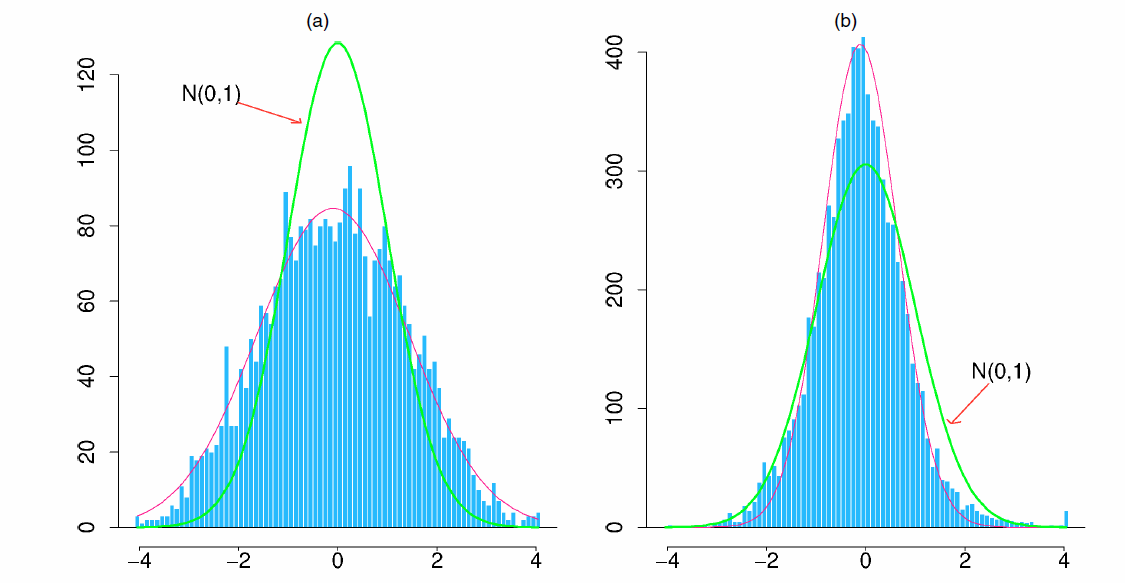
\includegraphics[scale=0.35]{efron2007figure1}
	\caption{ \footnotesize{Histograms of z-Values From Two Microarray Experiments. (a) Breast cancer study, 3,226 genes. (b) HIV study, 7,680 genes. Heavy curves indicate N(0, 1) theoretical null densities; Light curves indicate empirical null densities fit to central z-values, as done by Efron (2004). The theoretical null distributions are too narrow in (a) and too wide in (b). Both effects can be caused by correlations among the null z-values.}}
	\label{fig1}
\end{figure}
\end{frame}

\begin{frame}[t]{Introduction}\vspace{10pt}
Correlation can cause effects like those shown in Figure \ref{fig1}, considerably widening or narrowing the distribution of the null $z$-values.

These effects have a substantial impact on simultaneous significance testing and must be accounted for in deciding which cases should be reported as nonnull.

Broadly speaking, a wide central histogram like that for the breast cancer data implies more null $z$-values in the tails, so that significance levels judged according to the theoretical $N(0, 1)$ null are too liberal. Conversely, the theoretical null is too conservative for the HIV data.

\end{frame}

\begin{frame}[t]{Introduction}\vspace{10pt}
A surprisingly simple result emerges in which the main effect of all the pairwise correlations (several million of them for Fig. 1’s examples) is summarized by a single dispersion variate, A: 

a positive value of A widens the central peak of the z-value histogram, even assuming that the theoretical null (\ref{eq2}) is individually correct for all the cases, whereas negative A narrows it, as in Figure \ref{fig1}(b).
\end{frame}

\begin{frame}[t]{Introduction}\vspace{10pt}
\begin{figure}[h]
	\centering
	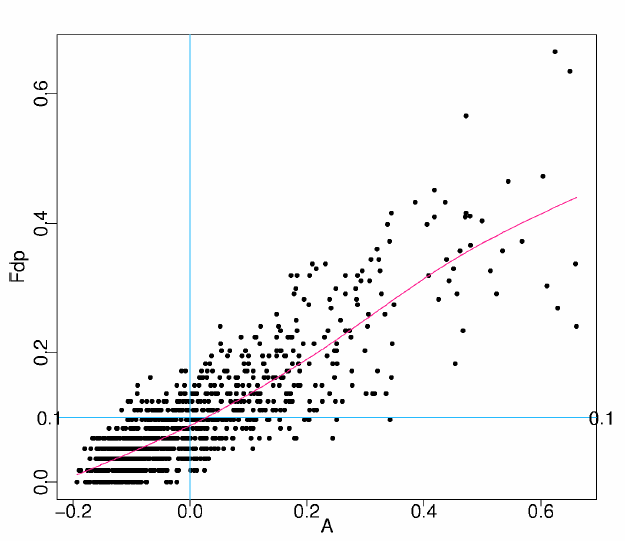
\includegraphics[scale=0.35]{efron2007figure2}
	\caption{ \footnotesize{Benjamini–Hochberg FDR Controlling Procedure, $q = .10$,Run for $1,000$ Simulation Trials; True False Discovery Proportion, FDP, Plotted versus Dispersion Variate $A$. Overall FDP averaged $.096$, close to $q$, but with a strong dependence on $A$, as shown by smooth regression curve.}}
	\label{fig2}
\end{figure}
\end{frame}

\begin{frame}[t]{Introduction}\vspace{10pt}
We see a strong dependence on the dispersion variate $A$; FDP averaged $.34$ for the upper $5\%$ of $A$ realizations but only $.03$ for the lower $5\%$.

$A$ can be estimated from the width of the central peak of the $z$-value histogram; narrow peaks imply negative $A's$ and wide peaks imply positive $A's$.

In terms of Figure \ref{fig2}, this enables the statistician to condition the $FDR$ estimate on its approximate location along the $A$ axis.
\end{frame}

\begin{frame}[t]{Introduction}\vspace{10pt}

\end{frame}

\begin{frame}[t]{Correlation effects on the null distribution}\vspace{10pt}
For following calculations, it is assumed that all cases are null,
\begin{equation}\label{eq3}
Z_i \sim N(0,1), \qquad  for \ i=1,2,...,N
\end{equation}

It is helpful to work with histogram counts rather than with the vector of $z$-values itself. Each histogram in Figure \ref{fig1} has its $z$-axis partitioned into $K = 82$ bins of width $\Delta = .1$, running from $−4.1 to 4.1$.

\end{frame}

\begin{frame}[t]{Correlation effects on the null distribution}\vspace{10pt}
We denote the count vector by $y$,

\begin{equation}\label{eq4}
y_k = \#\{z_i \ in \ kth \ bin \}, \qquad k=1,2,...,K
\end{equation}

The histogram counts $y_k$ arise from a partition of Z into $K$ bins,

\begin{equation}\label{eq5}
Z = \bigcup_{k=1}^K z_k,	
\end{equation}
each bin being of width $\Delta$, with center point $"z[k]"$

\end{frame}


\begin{frame}[t]{Correlation effects on the null distribution}\vspace{10pt}
The following definitions lead to useful representations for the mean and covariance of $y$.
\begin{equation}\label{eq6}
\pi_k(i) = Pr\{z_i \in Z_k \}, \qquad \pi_{k\cdot}=\frac{\sum_{i=1}^N \pi_k(i)}{N}
\end{equation}

\begin{equation}\label{eq7}
\gamma_{kl}(i,j) = Pr \{z_i \in Z_k \ and \ z_j \in Z_l \}, \qquad
\gamma_{kl\cdot}=\frac{\sum_{i \neq j} \gamma_{kl}(i,j) } {N(N-1)}.
\end{equation}

\end{frame}

\begin{frame}[t]{Correlation effects on the null distribution}\vspace{10pt}
Because of assumption (\ref{eq3}), all of the $\pi_k(i)$ are determined by $\varphi(z)$, the standard normal density, with Taylor approximation around centerpoint $z[k]$,

\begin{equation}\label{eq8}
\pi_{k\cdot}= \pi_k(i) \doteq  \Delta \cdot \varphi(z[k])
\end{equation}

The expectation vector, $\textbf{v} = (v_1, v_2, . . . , v_K)'$ of $y$ is determined by (\ref{eq3}),

\begin{equation}\label{eq9}
\textbf{v} = N \boldsymbol{\pi.}\doteq (...,N\Delta\varphi(z[k]),...)'.
\end{equation}

\end{frame}

\begin{frame}[t]{Correlation effects on the null distribution}\vspace{10pt}
\textbf{\textit{Lemma 1}}

\begin{equation}\label{eq10}
cov(\boldsymbol{y}) = C_0 +C_1
\end{equation}

\begin{equation}\label{eq11}
C_0 = diag(\boldsymbol{v}) - \boldsymbol{v}\boldsymbol{v'}/N = N[diag(\boldsymbol{\pi.}) - \boldsymbol{\pi.}\boldsymbol{\pi.'}]
\end{equation}

\begin{equation}\label{eq12}
C_1 = (1-\frac{1}{N})diag(\boldsymbol{v})\boldsymbol{\delta}diag(\boldsymbol{v}), \quad with \ \delta_{kl} = \gamma_{kl.}/\pi_{k.}\pi_{l.} -1
\end{equation}
\end{frame}

\begin{frame}[t]{Correlation effects on the null distribution}\vspace{10pt}
If $z_i$ and $z_j$ are independent, then$\gamma_{kl}(i,j)=\pi_{k}(i)\pi_{j}(l)$. Independence of all $z$-values implies that all of the elements of matrix $\boldsymbol{\delta}$ in (\ref{eq12}) are 0, leaving $cov(y) = C_0$.

Conversely, the amount of correlation between the $z$-values determines the size of $\boldsymbol{\delta}$ and the increase of $cov(y)$ above $C_0$.


\end{frame}

\begin{frame}[t]{Correlation effects on the null distribution}\vspace{10pt}
To approximate $\boldsymbol{\delta}$, we add the assumption of bivariate normality for any pair of $z$-values, $cov(z_i, z_j) \equiv \rho_{ij}$. 

Let $g(\rho)$ indicate the empirical density of the $N(N-1)$ correlations $\rho_{ij}$

\textbf{\textit{Lemma 2}} Under the bivariate normal approximation, the matrix $\boldsymbol{\delta}$ has elements

\begin{equation}\label{eq13}
\begin{split}
\delta_{kl}  \doteq & \int_{-1}^{1}\int_{-1}^{1} [\frac{1}{\sqrt{1-\rho^2}}exp(\frac{\rho}{2(1-\rho^2)}\times \{2z[k]z[l] - \\
& \rho(z[k]^2+z[l]^2)\} ) -1  ] g(\rho)d\rho
\end{split}
\end{equation}

\end{frame}

\begin{frame}[t]{Correlation effects on the null distribution}\vspace{10pt}
Application of Lemmas 1 and 2 reqires estimation of the correlation density $g(\rho)$, which we can obtain from observed correlations between the rows of $X$.

\begin{equation}\label{eq14}
breast cancer: \ g(\rho) \dot{\sim} N(0,.153^2)
\end{equation}

\begin{equation}\label{eq15}
HIV: \ g(\rho) \dot{\sim} N(0,.42^2)
\end{equation}

Approximation (\ref{eq14}) indicates a substantial amount of global correlation among genes in the breast cancer study, and even more correlation for the HIV study.

\end{frame}

\begin{frame}[t]{First Eigenvector}\vspace{10pt}
Lemmas 1 and 2 decompose the covariance matrix of the count vector $y$ into an independence term $C_0$ and an additional term $C_1$ that accounts for correlation among the z-values.

This section presents a simple approximation to $C_1$ in terms of its first eigenvector,

\end{frame}

\begin{frame}[t]{First Eigenvector}\vspace{10pt}
\textbf{\textit{Lemma 3}} Suppose that $g(\rho)$, the correlation density in (\ref{eq13}) has mean 0 and standard deviation
\begin{equation}\label{eq16}
\alpha = \left[\int_{-1}^1\rho^2g(\rho)d\rho\right]^{-1/2}
\end{equation}
Then the matrix $\boldsymbol{\delta}$ in (\ref{eq12}) is approximated by the outer product

\begin{equation}\label{eq17}
\boldsymbol{\delta} \doteq \alpha^2\boldsymbol{q}\boldsymbol{q'}, \ where \ q_k = \frac{z[k]^2-1}{\sqrt{2}}
\end{equation}

\end{frame}


\begin{frame}[t]{First Eigenvector}\vspace{10pt}

\begin{figure}[h]
	\centering
	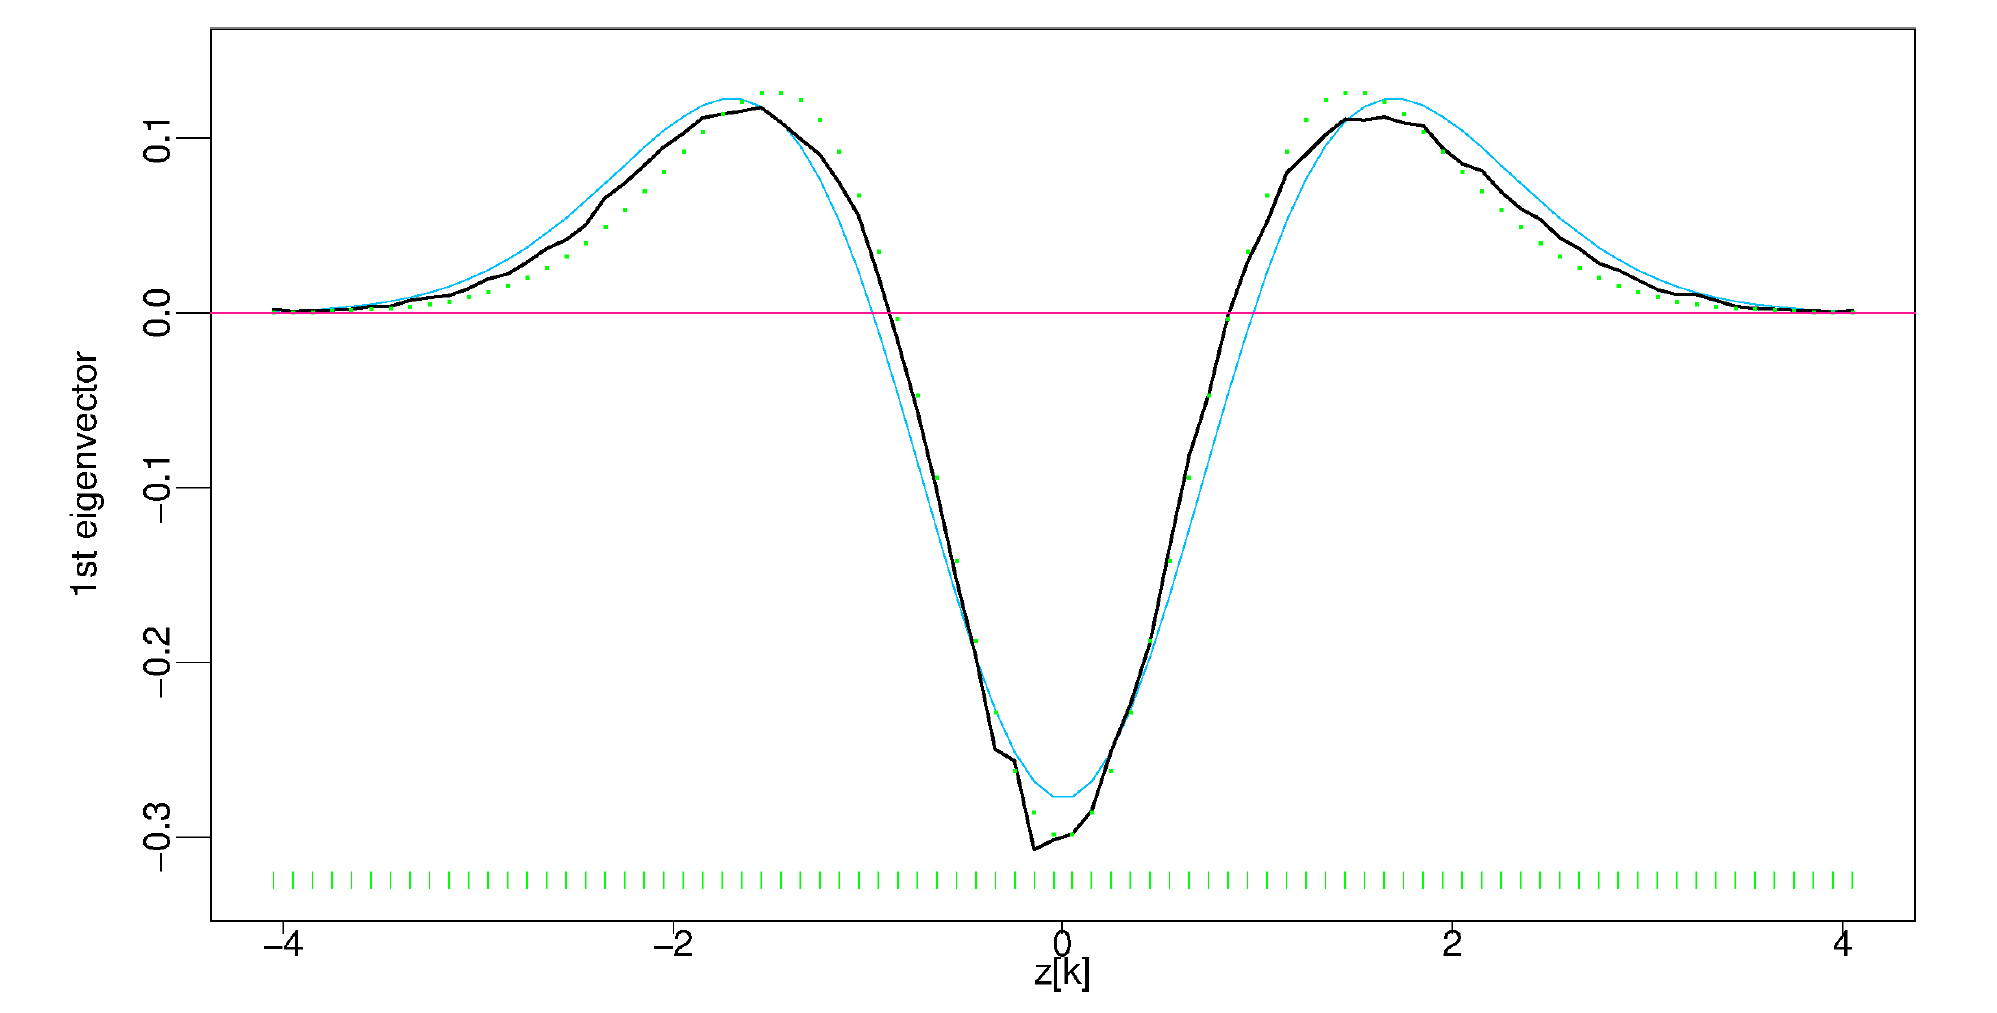
\includegraphics[scale=0.35]{efron2007figure3}
	\caption{\footnotesize{First Eigenvectors of Three Different Estimates of $cov(y)$: Normal-Theory Estimate for Breast Cancer Data (smooth curve); Normal-Theory Estimate for HIV Data (dots), and Permutation Estimate for Breast Cancer Data (jagged curve). The striking 'wing-shaped' form is proportional to the second derivative of the standard normal density.}}
	\label{fig3}
\end{figure}

\end{frame}


\begin{frame}[t]{First Eigenvector}\vspace{10pt}
Combining the three lemmas yields a useful approximation for the null covariance matrix of the count vector $\boldsymbol{y}$ under the bivariate normal assumptions.

\textbf{\textit{Theorem}} If $g(\rho)$ has mean 0 and standard deviation $\alpha$, then 

\begin{equation}\label{eq18}
cov(\boldsymbol{y}) \doteq [diag(\boldsymbol{v}) - \boldsymbol{v}\boldsymbol{v'}/N] + \left(1-\frac{1}{N}\right)(\alpha\boldsymbol{W})(\alpha\boldsymbol{W})',
\end{equation}

Here $\boldsymbol{v} = E\{\boldsymbol{y}\}$, $\boldsymbol{W}$ has components

\begin{equation}\label{eq19}
W_k = N\Delta\varphi(z[k])\frac{z[k]^2-1}{\sqrt{2}} =  N\Delta w(z[k])
\end{equation}
The Theorem summarizes the effect of $z's$ entire correlation structure in a single parameter $\alpha$.
\end{frame}

\begin{frame}[t]{Poisson process}\vspace{10pt}
Poisson process considerations lead to a somewhat rough but evocative interpretation of the Theorem. Let $\boldsymbol{y}\sim Po(\boldsymbol{u})$ indicate a vector of independent Poisson variates, $y_k \stackrel{ind}{\sim} Po(u_k)$ for $k=1,2,...,K$, whereas $\boldsymbol{y} \sim (\boldsymbol{v}, \Gamma)$ denotes that vector $\boldsymbol{v}$ has mean $\boldsymbol{v}$ and covariance $\Gamma$.

\end{frame}

\begin{frame}[t]{Poisson process}\vspace{10pt}
Consider the number of cases $N$ to be a Poisson variate, say

\begin{equation}\label{eqpo1}
N \sim Po(N_0),
\end{equation}

with $N_0 = 3226$ in the breast cancer study. This simplifies (\ref{eq18}) slightly, to
\begin{equation}\label{eqpo2}
cov(\boldsymbol{y}) \doteq diag(\boldsymbol{v})  + (\alpha\boldsymbol{W})(\alpha\boldsymbol{W})'.
\end{equation}
If the $z$-values are independent, then (\ref{eqpo1}) makes the counts, $y_k$,independent Poisson variates,
\begin{equation}\label{eqpo3}
\boldsymbol{y} \sim Po(\boldsymbol{v}), \ agreeing \ with \ (\ref{eqpo2})\  at \ \alpha = 0.
\end{equation}
\end{frame}

\begin{frame}[t]{Poisson process}\vspace{10pt}
A hierarchical model generalizes (\ref{eqpo3}) to incorporate dependence. We assume that $\boldsymbol{y}$ depends on a mean vector $\boldsymbol{u}$, itself random,

\begin{equation}\label{eqpo4}
\boldsymbol{y}|\boldsymbol{u} \sim Po(\boldsymbol{u}), \ where \  \boldsymbol{u}\sim (\boldsymbol{v}, \Gamma),
\end{equation}
so that the components of $\boldsymbol{y}$ are conditionally independent given
$\boldsymbol{u}$ but marginally dependent, with mean and covariance

\begin{equation}\label{eqpo5}
\boldsymbol{y}\sim (\boldsymbol{v}, diag(\boldsymbol{v})+\Gamma).
\end{equation}

To match (\ref{eqpo2}), we set
\begin{equation}\label{eqpo6}
\Gamma = (\alpha\boldsymbol{W})(\alpha\boldsymbol{W})'.
\end{equation}

\end{frame}


\begin{frame}[t]{Poisson process}\vspace{10pt}
Formulas (\ref{eqpo5}) and (\ref{eqpo6}) suggest a hierarchical Poisson structure for the count vector $\boldsymbol{y}$,

\begin{equation}\label{eqpo7}
\boldsymbol{y}\sim Po(\boldsymbol{u}), where \ \boldsymbol{u} = \boldsymbol{v} + A\boldsymbol{W}, with \ A \sim(0,\alpha^2)
\end{equation}
If $\alpha = 0$, then this reduces to the independence case (\ref{eqpo3}); otherwise, the Poisson intensity vector $\boldsymbol{v}$ is modified by the addition of an independent random multiple $A$ of $\boldsymbol{W}$ with standard deviation $\alpha$.
\end{frame}


\begin{frame}[t]{Large-scale Significance Testing}\vspace{10pt}
Suppose for a moment that we knew which $z_i's$ among the full set of $z$-values correspond to null cases. For a given choice of $x$, define

\begin{equation}\label{eq20}
Y(x)= \# \{null \ z_i \geq x\} \quad T(x)= \# \{z_i \geq x\} 
\end{equation}

\begin{equation}\label{eq21}
FDR(x) = E\{Y(x)\}/T(x).
\end{equation}
FDR(x) is an empirical Bayes estimate of the a posteriori probability that case $i$ is null given $z_i \geq x$, amounting to a version of Storey's "q-value".
\end{frame}


\begin{frame}[t]{Large-scale Significance Testing}\vspace{10pt}
The hierarchical structure gives conditional expectation 

\begin{equation}\label{eq22}
E\{\boldsymbol{y}|A\} = \boldsymbol{v}+ A\boldsymbol{W}
\end{equation}

Letting the bin width $\Delta \rightarrow 0$ produces a conditional version of (\ref{eq22})
\begin{equation}\label{eq23}
E\{Y(x)|A\} = N\bar{\Phi}(x) \left[ 1+A\frac{x\varphi(x)}{\sqrt{2}\bar{\Phi}(x)} \right]
\end{equation}

Conditional FDR
\begin{equation}\label{eq24}
FDR(Y(x)|A) = FDR_0(x)\left[1+A\frac{x\varphi(x)}{\sqrt{2}\bar{\Phi}(x)} \right],
\end{equation}
where $FDR_0(x)$ is the standard unconditional estimate $N\bar{\Phi}(x)/T(x)$ based on the theoretical $N(0, 1)$ null.
\end{frame}

\begin{frame}[t]{Large-scale Significance Testing}\vspace{10pt}
A can be estimated from the central spread of the histogram of $z$-values and then used to condition inferences, as in figure \ref{fig2}.

For $x_0 > 0$, let 

\begin{equation}\label{eq25}
Y_0 = \#\{z_i \in [-x0,x0]\},
\end{equation}
and define
\begin{equation}\label{eq26}
P_0 =2\Phi(x_0) -1  \quad and \ Q_0 =\sqrt{2}x_0\varphi(x0)
\end{equation}
Then (\ref{eq23}) give $E\{Y_0|A\} \doteq N[P_0-AQ_0]$, so

\begin{equation}\label{eq27}
\hat{A} = \frac{P_0 - \hat{P}_0}{Q_0}, \ where\ \hat{P}_0 = Y_0/N
\end{equation}

\end{frame}

\begin{frame}[t]{Large-scale Significance Testing}\vspace{10pt}
We could substitute $\hat{A}$ from (\ref{eq27}) into (\ref{eq24}) to obtain a conditional FDR estimate,


\begin{equation}\label{eq28}
FDR(x|\hat{A}) = FDR_0(x)\left[1+\hat{A}\frac{x\varphi(x)}{\sqrt{2}\bar{\Phi}(x)} \right],
\end{equation}

\vspace{0.7cm}

In situations like that of Figure \ref{fig2}, the goal would be to accurately assess our position on the $A$ axis, to better estimate $FDP$ rather than estimating the unconditional average of $FDP$.
\end{frame}

\begin{frame}[t]{Large-scale Significance Testing}\vspace{10pt}
\begin{figure}[h]
	\centering
	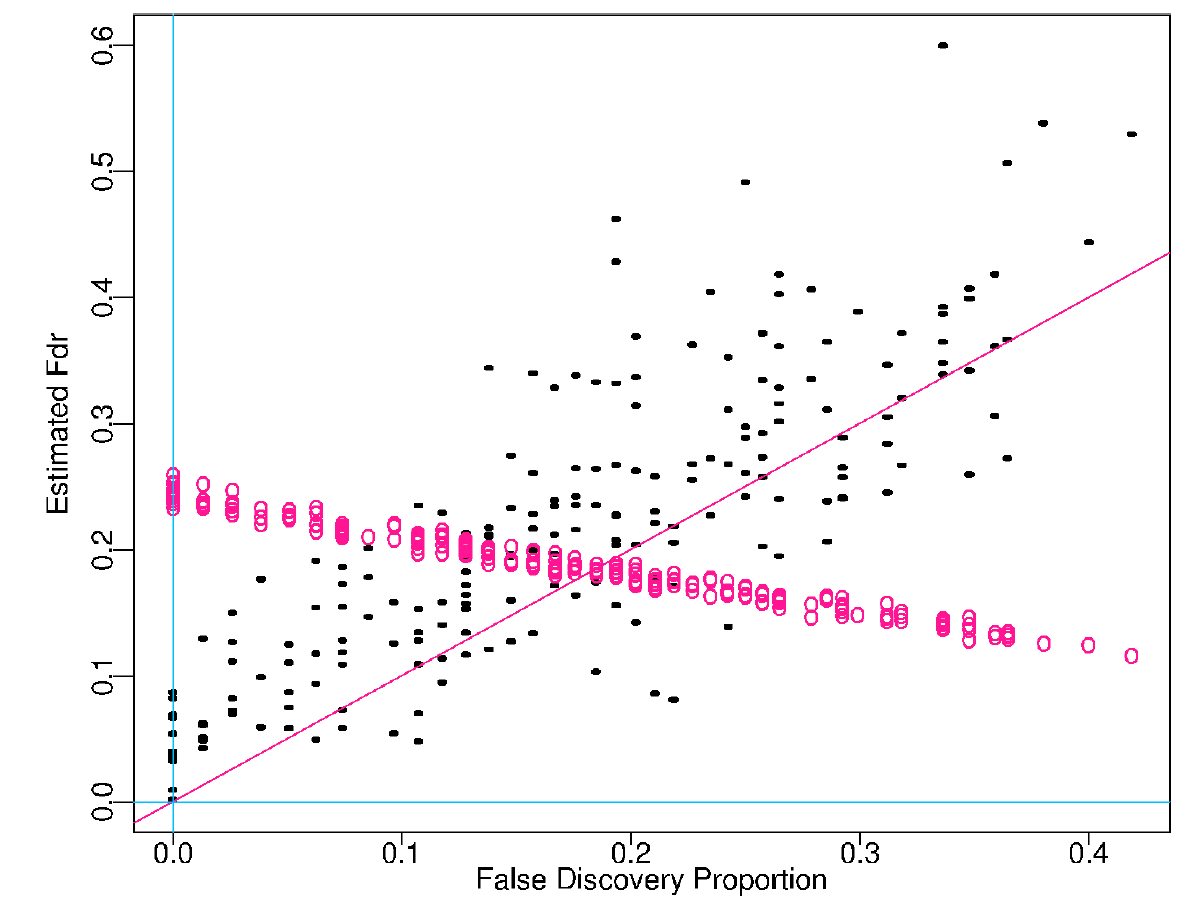
\includegraphics[scale=0.35]{efron2007figure4}
	\caption{\footnotesize{Simulation Experiment Comparing Conditional FDR Estimates (solid points), With Unconditional Estimates (open circles); N = 3,000, p0 = .95. Null counts are generated as in (\ref{eqpo7}), $\alpha$ = .15; nonnull counts from $z \sim N(2.5, 1.25)$. The horizontal axis is the actual FDP, FDP(x), x = 2.5, for each of the 200 trials. The unconditional estimate based on the theoretical null distribution declines as actual FDP increases.}}
	\label{fig4}
\end{figure}

\end{frame}


\begin{frame}[t]{Large-scale Significance Testing}\vspace{10pt}

Strikingly, the unconditional estimate goes in the wrong direction, declining as the actual $FDP$ increases. This yields misleading inferences at both ends of the $FDP$ scale. The conditional $FDR$ estimate correctly tracks FDP, although with a considerable amount of noise.

\end{frame}


\end{document}